% Conceptual Framework v2 — abstraction-first.
% Panel A: 3 entity clouds (Commuters / Places / Transport Network) with icon
%          attributes, plus emergent aggregate flow F_{ij,t}.
% Panel B: 4 trade-off cards (time / distance / job match / income) revealed
%          by the conceptual lens, with a counterfactual reasoning prompt.
%
% No "real world" cartoon panel, no encoder / RUM / BPR / Stage 1-2 jargon.
%
% Compile: pdflatex figure_conceptual_v2.tex

\documentclass[border=10pt]{standalone}

\usepackage[T1]{fontenc}
\usepackage{lmodern}
\usepackage{amsmath, amssymb}
\usepackage{tikz}
\usepackage{xcolor}

\usetikzlibrary{
  positioning, arrows.meta, shapes.geometric, shapes.symbols, shapes.misc,
  calc, fit, backgrounds, decorations.pathmorphing,
}

% ── Soft colour palette ────────────────────────────────────────────────
\definecolor{cCommBg}     {HTML}{E0F2FE}    % light blue — commuters
\definecolor{cCommBorder} {HTML}{0369A1}
\definecolor{cPlacesBg}   {HTML}{FEF3C7}    % light amber — places
\definecolor{cPlacesBorder}{HTML}{B45309}
\definecolor{cNetBg}      {HTML}{D1FAE5}    % light green — network
\definecolor{cNetBorder}  {HTML}{047857}
\definecolor{cFlowBg}     {HTML}{FAE5DD}    % salmon — emergent flow
\definecolor{cFlowBorder} {HTML}{C44E52}
\definecolor{cTradeBg}    {HTML}{F3E8FF}    % light purple — trade-offs
\definecolor{cTradeBorder}{HTML}{6D28D9}

\definecolor{cTime}       {HTML}{C44E52}
\definecolor{cDist}       {HTML}{F59E0B}
\definecolor{cMatch}      {HTML}{0E7490}
\definecolor{cTier}       {HTML}{8172B2}

\definecolor{cText}       {HTML}{1F2937}
\definecolor{cMuted}      {HTML}{6B7280}
\definecolor{cFlow}       {HTML}{E07A5F}
\definecolor{cQuestion}   {HTML}{8172B2}

\definecolor{cAgentWalk}    {HTML}{10B981}
\definecolor{cAgentTransit} {HTML}{F59E0B}
\definecolor{cAgentCar}     {HTML}{3B82F6}
\definecolor{cTierLow}      {HTML}{93C5FD}
\definecolor{cTierMid}      {HTML}{C4B5FD}
\definecolor{cTierHigh}     {HTML}{F0ABFC}

\begin{document}

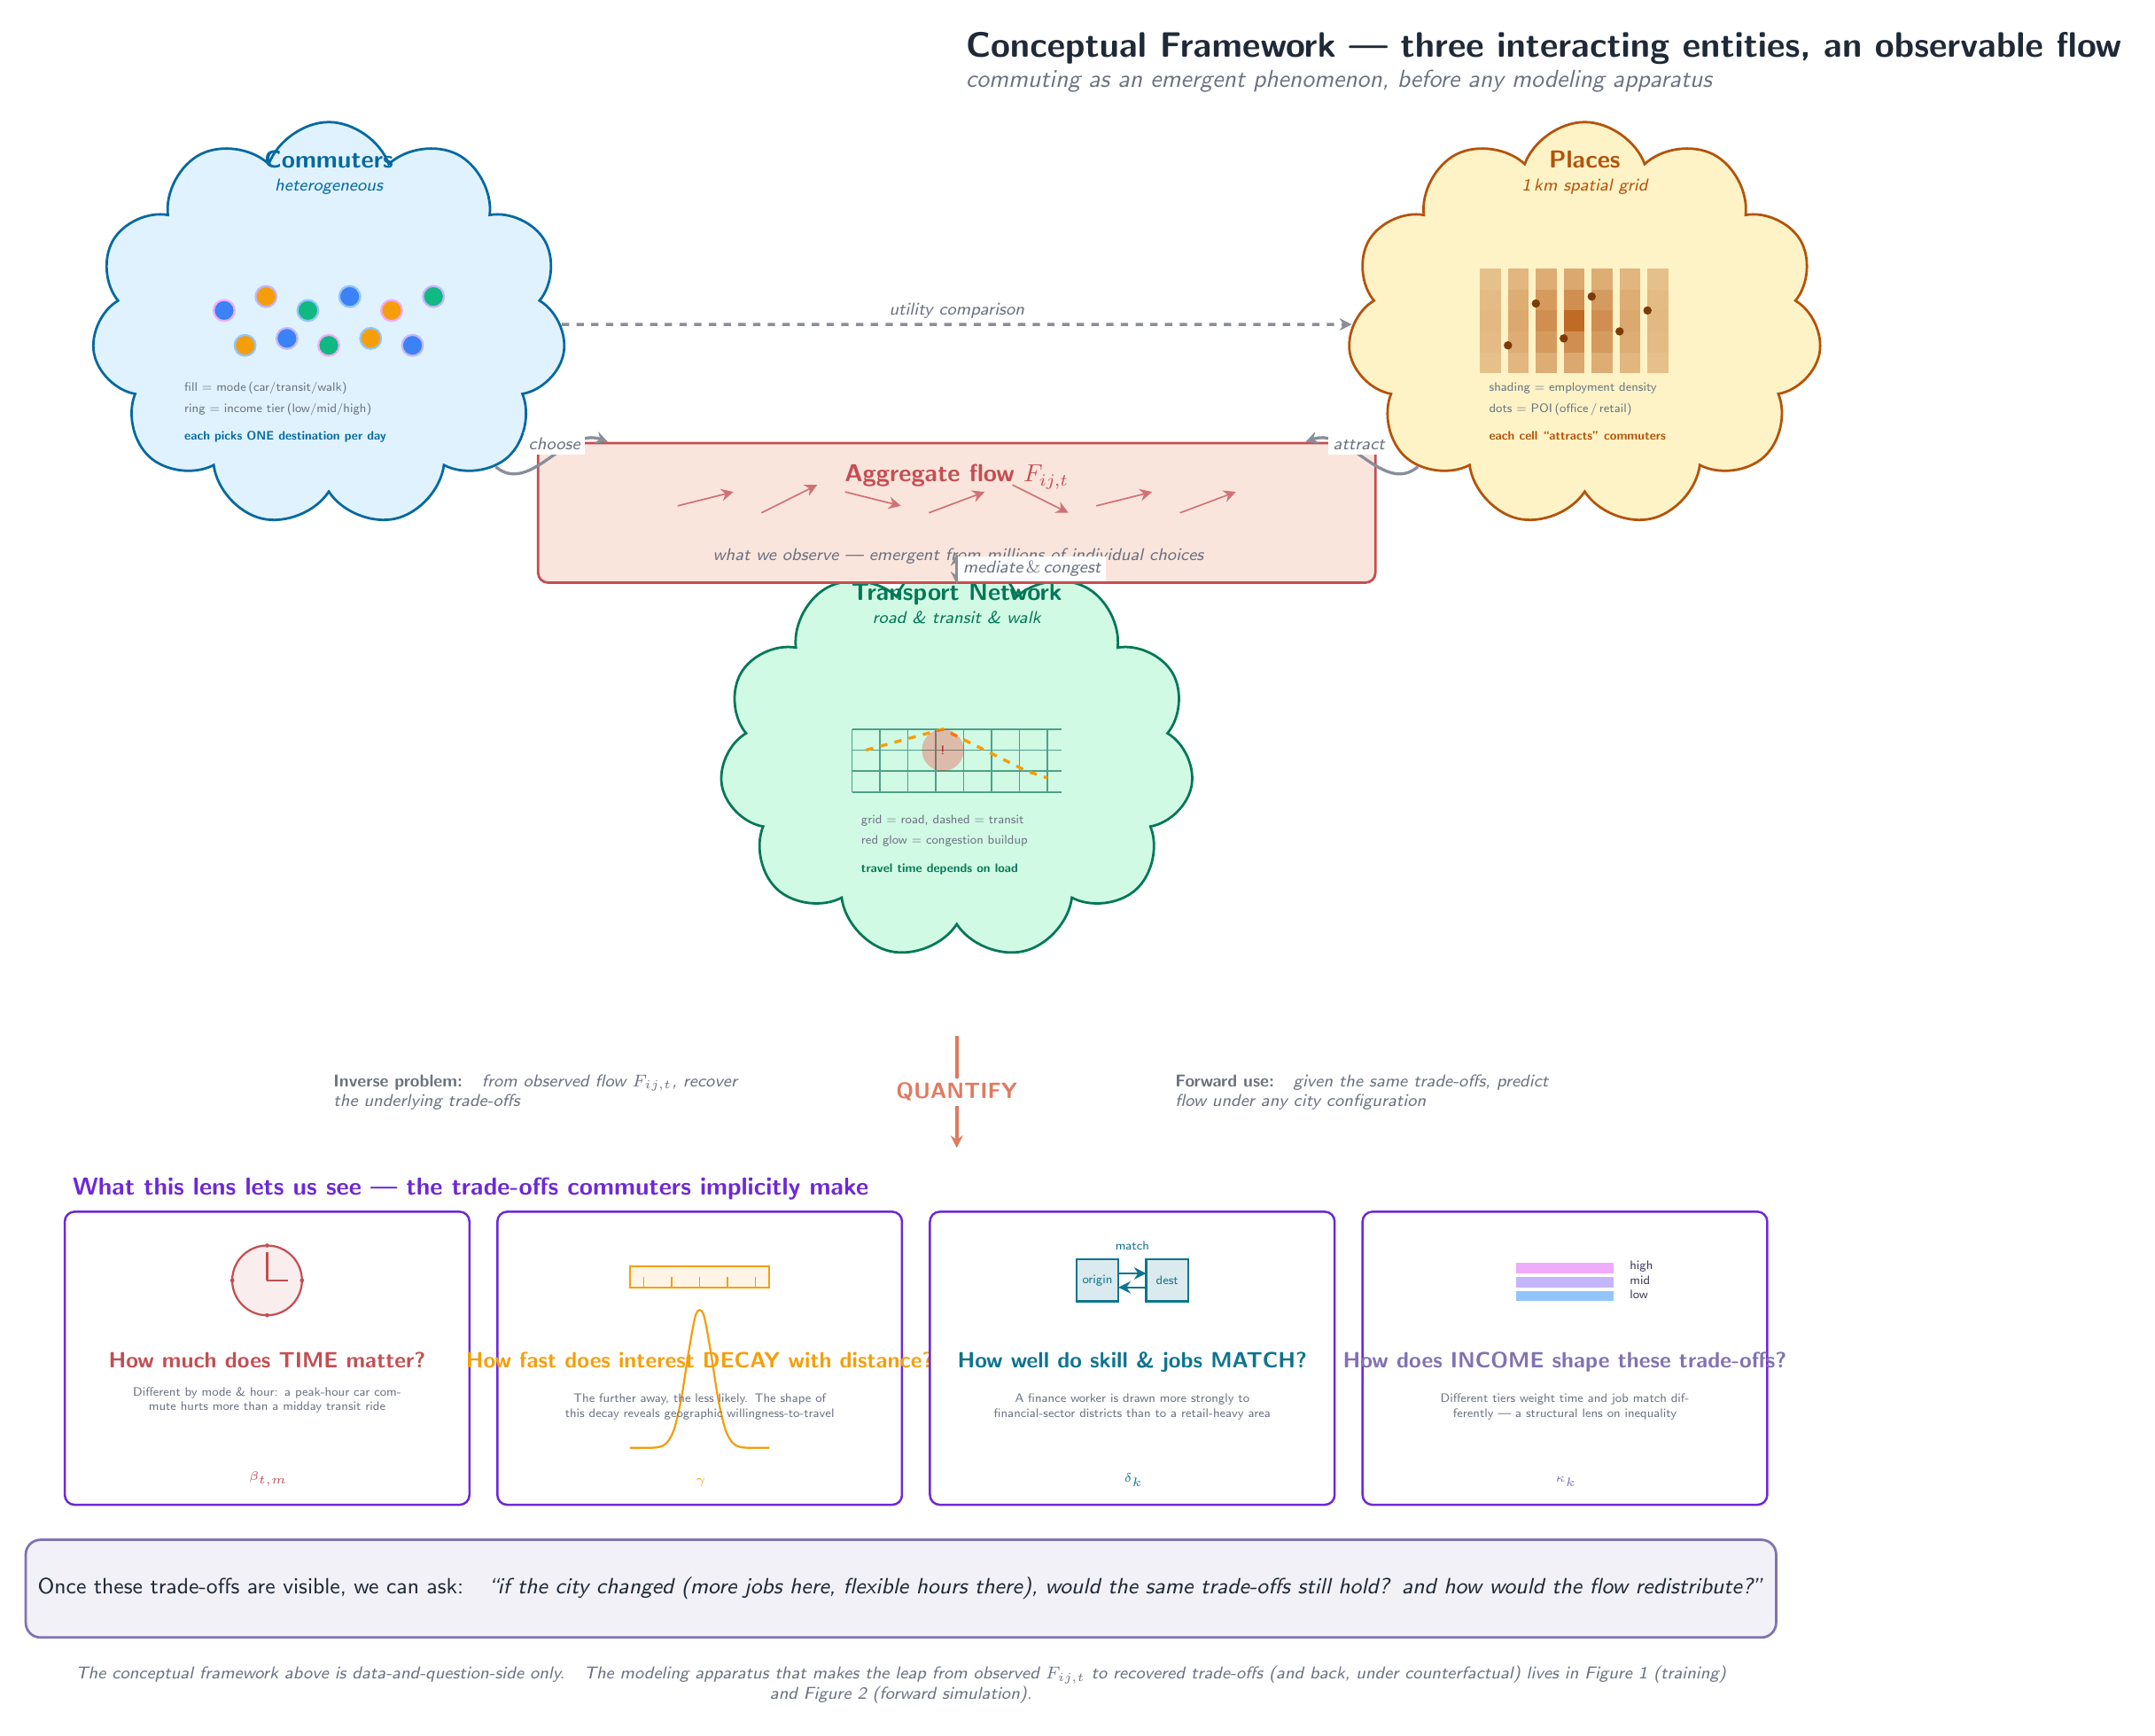
\begin{tikzpicture}[
  font=\sffamily,
  thick,
  >={Stealth[length=5pt, width=5pt]},
  every node/.style={align=center, text=cText},
  cloudCommuter/.style={
    cloud, cloud puffs=11, cloud puff arc=140,
    draw=cCommBorder, fill=cCommBg, line width=1.0pt,
    minimum width=68mm, minimum height=58mm, aspect=1.2,
    font=\sffamily\small,
  },
  cloudPlaces/.style={
    cloud, cloud puffs=11, cloud puff arc=140,
    draw=cPlacesBorder, fill=cPlacesBg, line width=1.0pt,
    minimum width=68mm, minimum height=58mm, aspect=1.2,
    font=\sffamily\small,
  },
  cloudNet/.style={
    cloud, cloud puffs=11, cloud puff arc=140,
    draw=cNetBorder, fill=cNetBg, line width=1.0pt,
    minimum width=68mm, minimum height=58mm, aspect=1.2,
    font=\sffamily\small,
  },
  flowbox/.style={
    rectangle, rounded corners=4pt,
    draw=cFlowBorder, fill=cFlowBg, line width=1.0pt,
    minimum width=120mm, minimum height=20mm,
    font=\sffamily\small,
  },
  tradecard/.style={
    rectangle, rounded corners=4pt,
    draw=cTradeBorder, fill=white, line width=0.9pt,
    minimum width=58mm, minimum height=42mm,
    font=\sffamily\footnotesize,
  },
  arrAct/.style={->, line width=1.2pt, draw=cMuted!80},
  arrEmerge/.style={->, line width=1.4pt, draw=cFlow},
  arrlbl/.style={font=\sffamily\scriptsize\itshape, text=cMuted, fill=white,
                 inner sep=2pt},
]

% ════════════════════════════════════════════════════════════════════════
%  PANEL A — Conceptual Lens (3 entity clouds + emergent flow)
% ════════════════════════════════════════════════════════════════════════

% ── Title ─────────────────────────────────────────────────────────────
\node[font=\sffamily\bfseries\Large, anchor=south west, text=cText]
  at (0, 60mm)
  {Conceptual Framework — three interacting entities, an observable flow};
\node[font=\sffamily\itshape\normalsize, anchor=south west, text=cMuted]
  at (0, 56mm)
  {commuting as an emergent phenomenon, before any modeling apparatus};

% ── COMMUTERS cloud (top-left) ────────────────────────────────────────
\node[cloudCommuter] (commuters) at (-90mm, 24mm) {};
\node[font=\sffamily\bfseries\normalsize, text=cCommBorder, anchor=north]
  at ($(commuters.north)+(0,-3mm)$) {Commuters};
\node[font=\sffamily\scriptsize\itshape, text=cCommBorder, anchor=north]
  at ($(commuters.north)+(0,-7mm)$) {heterogeneous};

% Commuters icon: dots colored by mode + tier
\begin{scope}[shift={(commuters.center)}]
  % a small grid of agents — each a circle, color = mode, ring = tier
  \foreach \i/\dx/\dy/\modeC/\tierC in {
    1/-15/2/cAgentCar/cTierHigh,
    2/-9/4/cAgentTransit/cTierMid,
    3/-3/2/cAgentWalk/cTierLow,
    4/3/4/cAgentCar/cTierLow,
    5/9/2/cAgentTransit/cTierHigh,
    6/15/4/cAgentWalk/cTierMid,
    7/-12/-3/cAgentTransit/cTierLow,
    8/-6/-2/cAgentCar/cTierMid,
    9/0/-3/cAgentWalk/cTierHigh,
    10/6/-2/cAgentTransit/cTierLow,
    11/12/-3/cAgentCar/cTierMid}{
    \draw[draw=\tierC, fill=\modeC, line width=0.8pt]
          (\dx mm, \dy mm) circle (1.5mm);
  }
  % small legend
  \node[font=\sffamily\tiny, text=cMuted, anchor=north west]
    at (-22mm, -7mm) {fill = mode\,(car/transit/walk)};
  \node[font=\sffamily\tiny, text=cMuted, anchor=north west]
    at (-22mm, -10mm) {ring = income tier\,(low/mid/high)};
  \node[font=\sffamily\tiny, text=cCommBorder, anchor=north west]
    at (-22mm, -14mm) {\textbf{each picks ONE destination per day}};
\end{scope}

% ── PLACES cloud (top-right) ──────────────────────────────────────────
\node[cloudPlaces] (places) at (90mm, 24mm) {};
\node[font=\sffamily\bfseries\normalsize, text=cPlacesBorder, anchor=north]
  at ($(places.north)+(0,-3mm)$) {Places};
\node[font=\sffamily\scriptsize\itshape, text=cPlacesBorder, anchor=north]
  at ($(places.north)+(0,-7mm)$) {1\,km spatial grid};

% Places icon: small grid with employment heatmap + POI dots
\begin{scope}[shift={(places.center)}]
  \foreach \r in {0,1,2,3,4}{
    \foreach \c in {0,1,2,3,4,5,6}{
      % concentric attractiveness — peak at center
      \pgfmathsetmacro{\dist}{sqrt((\c-3)*(\c-3) + (\r-2)*(\r-2))}
      \pgfmathsetmacro{\op}{0.15 + 0.7*exp(-0.4*\dist)}
      \fill[cPlacesBorder, opacity=\op]
            (-15mm + \c*4mm, 5mm - \r*3mm) rectangle
            (-12mm + \c*4mm, 8mm - \r*3mm);
    }
  }
  % a few POI dots (offices)
  \foreach \dx/\dy in {-7/3, 1/4, 5/-1, -3/-2, 9/2, -11/-3}{
    \fill[cPlacesBorder!70!black] (\dx mm, \dy mm) circle (0.6mm);
  }
  \node[font=\sffamily\tiny, text=cMuted, anchor=north west]
    at (-15mm, -7mm) {shading = employment density};
  \node[font=\sffamily\tiny, text=cMuted, anchor=north west]
    at (-15mm, -10mm) {dots = POI\,(office\,/\,retail)};
  \node[font=\sffamily\tiny, text=cPlacesBorder, anchor=north west]
    at (-15mm, -14mm) {\textbf{each cell ``attracts'' commuters}};
\end{scope}

% ── TRANSPORT NETWORK cloud (bottom) ──────────────────────────────────
\node[cloudNet] (network) at (0, -38mm) {};
\node[font=\sffamily\bfseries\normalsize, text=cNetBorder, anchor=north]
  at ($(network.north)+(0,-3mm)$) {Transport Network};
\node[font=\sffamily\scriptsize\itshape, text=cNetBorder, anchor=north]
  at ($(network.north)+(0,-7mm)$) {road \& transit \& walk};

% Network icon: simplified street/transit graph + congestion glow
\begin{scope}[shift={(network.center)}]
  % road grid (gray)
  \foreach \r in {0,1,2,3}{
    \draw[draw=cNetBorder!70, line width=0.6pt]
          (-15mm, 4mm - \r*3mm) -- (15mm, 4mm - \r*3mm);
  }
  \foreach \c in {0,1,2,3,4,5,6,7}{
    \draw[draw=cNetBorder!70, line width=0.6pt]
          (-15mm + \c*4mm, 4mm) -- (-15mm + \c*4mm, -5mm);
  }
  % transit line (dashed)
  \draw[draw=cAgentTransit, line width=1.2pt, dashed]
        (-13mm, 1mm) -- (-2mm, 4mm) -- (10mm, -2mm) -- (13mm, -3mm);
  % a "congestion hotspot" highlight at center intersection
  \fill[red, opacity=0.25] (-2mm, 1mm) circle (3mm);
  \node[font=\sffamily\tiny, text=red!70!black] at (-2mm, 1mm) {!};

  \node[font=\sffamily\tiny, text=cMuted, anchor=north west]
    at (-15mm, -7mm) {grid = road, dashed = transit};
  \node[font=\sffamily\tiny, text=cMuted, anchor=north west]
    at (-15mm, -10mm) {red glow = congestion buildup};
  \node[font=\sffamily\tiny, text=cNetBorder, anchor=north west]
    at (-15mm, -14mm) {\textbf{travel time depends on load}};
\end{scope}

% ── Aggregate flow box (center, between clouds) ──────────────────────
\node[flowbox] (flow) at (0, -3mm) {};
\node[font=\sffamily\bfseries\normalsize, text=cFlowBorder, anchor=north]
  at ($(flow.north)+(0,-2mm)$) {Aggregate flow $F_{ij,t}$};
\node[font=\sffamily\scriptsize\itshape, text=cMuted, anchor=south]
  at ($(flow.south)+(0,1.5mm)$)
  {\,what we observe — emergent from millions of individual choices};

% small flow arrows inside the flow box (suggestive)
\begin{scope}[shift={($(flow.center)+(0, 1mm)$)}]
  \foreach \dxa/\dya/\dxb/\dyb in {-40/0/-32/2, -28/-1/-20/3,
       -16/2/-8/0, -4/-1/4/2, 8/3/16/-1, 20/0/28/2, 32/-1/40/2}{
    \draw[->, line width=0.6pt, draw=cFlowBorder!80]
          (\dxa mm, \dya mm) -- (\dxb mm, \dyb mm);
  }
\end{scope}

% ── Relational arrows between clouds and flow ────────────────────────
% Commuters → Flow (choose)
\draw[arrAct] (commuters.south east) to[out=-40, in=160]
  node[arrlbl, pos=0.55, above]{choose}
  ($(flow.north)+(-50mm, 0)$);

% Places → Flow (attract)
\draw[arrAct] (places.south west) to[out=-140, in=20]
  node[arrlbl, pos=0.55, above]{attract}
  ($(flow.north)+(50mm, 0)$);

% Network ↔ Flow (mediate / congest)
\draw[arrAct, <->] (network.north) -- node[arrlbl, right]{mediate $\!\&\!$ congest}
  (flow.south);

% Commuters ↔ Places (information about each other)
\draw[arrAct, dashed] (commuters.east) -- node[arrlbl, above]{utility comparison}
  (places.west);

% ════════════════════════════════════════════════════════════════════════
%  Transition arrow + ABSTRACT/QUANTIFY label (between panels)
% ════════════════════════════════════════════════════════════════════════

% large downward "QUANTIFY" arrow
\draw[arrEmerge] (0, -78mm) -- (0, -94mm);
\node[font=\sffamily\bfseries\small, text=cFlow, fill=white, inner sep=2pt]
  at (0, -86mm) {QUANTIFY};

% Side annotations: inverse problem (left), forward (right)
\node[font=\sffamily\scriptsize\itshape, text=cMuted, anchor=east,
       text width=58mm, align=left]
  at (-30mm, -86mm)
   {\textbf{Inverse problem:}\;\;
    from observed flow $F_{ij,t}$, recover the underlying trade-offs};

\node[font=\sffamily\scriptsize\itshape, text=cMuted, anchor=west,
       text width=58mm, align=left]
  at (30mm, -86mm)
   {\textbf{Forward use:}\;\;
    given the same trade-offs, predict flow under any city configuration};

% ════════════════════════════════════════════════════════════════════════
%  PANEL B — What the lens lets us see (4 trade-off cards)
% ════════════════════════════════════════════════════════════════════════

\node[font=\sffamily\bfseries\normalsize, text=cTradeBorder, anchor=north west]
  at (-128mm, -97mm)
  {What this lens lets us see — the trade-offs commuters implicitly make};

% ⏰ TIME card
\node[tradecard, anchor=north west] (tcTime) at (-128mm, -103mm) {};
\begin{scope}[shift={($(tcTime.north)+(0,-4mm)$)}]
  % clock icon
  \draw[draw=cTime, fill=cTime!10, line width=0.8pt] (0, -6mm) circle (5mm);
  \draw[cTime, line width=0.8pt] (0, -6mm) -- (0, -2mm);   % minute hand
  \draw[cTime, line width=0.8pt] (0, -6mm) -- (3mm, -6mm); % hour hand
  \foreach \a in {0, 90, 180, 270}{
    \fill[cTime] ({\a}:5mm) ++ (0, -6mm) circle (0.3mm);
  }
\end{scope}
\node[font=\sffamily\bfseries\small, text=cTime, anchor=north]
  at ($(tcTime.north)+(0,-19mm)$) {How much does TIME matter?};
\node[font=\sffamily\tiny, text=cMuted, anchor=north,
       text width=52mm, align=center]
  at ($(tcTime.north)+(0,-24mm)$)
  {Different by mode \&\ hour: a peak-hour car commute hurts more than a midday transit ride};
\node[font=\sffamily\tiny\itshape, text=cTime, anchor=south]
  at ($(tcTime.south)+(0,1.5mm)$) {\,$\beta_{t,m}$};

% 📏 DISTANCE card
\node[tradecard, anchor=north west] (tcDist) at (-66mm, -103mm) {};
\begin{scope}[shift={($(tcDist.north)+(0,-4mm)$)}]
  % ruler icon — horizontal segmented bar
  \draw[draw=cDist, fill=cDist!10, line width=0.7pt] (-10mm, -7mm) rectangle (10mm, -4mm);
  \foreach \dx in {-8, -4, 0, 4, 8}{
    \draw[cDist, line width=0.5pt] (\dx mm, -7mm) -- (\dx mm, -5.5mm);
  }
  % decay curve overlay
  \draw[cDist, line width=0.8pt, smooth, samples=20, domain=-10:10]
        plot ({\x mm}, {2 * exp(-0.15*\x*\x) -3});
\end{scope}
\node[font=\sffamily\bfseries\small, text=cDist, anchor=north]
  at ($(tcDist.north)+(0,-19mm)$) {How fast does interest DECAY with distance?};
\node[font=\sffamily\tiny, text=cMuted, anchor=north,
       text width=52mm, align=center]
  at ($(tcDist.north)+(0,-25mm)$)
  {The further away, the less likely. The shape of this decay reveals geographic willingness-to-travel};
\node[font=\sffamily\tiny\itshape, text=cDist, anchor=south]
  at ($(tcDist.south)+(0,1.5mm)$) {\,$\gamma$};

% 🤝 OCC MATCH card
\node[tradecard, anchor=north west] (tcMatch) at (-4mm, -103mm) {};
\begin{scope}[shift={($(tcMatch.north)+(0,-4mm)$)}]
  % two interlocking shapes — origin SOC9 ↔ dest sector
  \draw[draw=cMatch, fill=cMatch!15, line width=0.8pt]
       (-8mm, -3mm) rectangle (-2mm, -9mm);
  \node[font=\sffamily\tiny, text=cMatch] at (-5mm, -6mm) {origin};
  \draw[draw=cMatch, fill=cMatch!15, line width=0.8pt]
       (2mm, -3mm) rectangle (8mm, -9mm);
  \node[font=\sffamily\tiny, text=cMatch] at (5mm, -6mm) {dest};
  % connect with arrows
  \draw[->, cMatch, line width=0.6pt] (-2mm, -5mm) -- (2mm, -5mm);
  \draw[<-, cMatch, line width=0.6pt] (-2mm, -7mm) -- (2mm, -7mm);
  \node[font=\sffamily\tiny, text=cMatch] at (0, -1mm) {match};
\end{scope}
\node[font=\sffamily\bfseries\small, text=cMatch, anchor=north]
  at ($(tcMatch.north)+(0,-19mm)$) {How well do skill \&\ jobs MATCH?};
\node[font=\sffamily\tiny, text=cMuted, anchor=north,
       text width=52mm, align=center]
  at ($(tcMatch.north)+(0,-25mm)$)
  {A finance worker is drawn more strongly to financial-sector districts than to a retail-heavy area};
\node[font=\sffamily\tiny\itshape, text=cMatch, anchor=south]
  at ($(tcMatch.south)+(0,1.5mm)$) {\,$\delta_k$};

% 💰 INCOME TIER card
\node[tradecard, anchor=north west] (tcTier) at (58mm, -103mm) {};
\begin{scope}[shift={($(tcTier.north)+(0,-4mm)$)}]
  % stacked income tier bars
  \fill[cTierLow] (-7mm, -9mm) rectangle (7mm, -7.5mm);
  \fill[cTierMid] (-7mm, -7mm) rectangle (7mm, -5.5mm);
  \fill[cTierHigh] (-7mm, -5mm) rectangle (7mm, -3.5mm);
  \node[font=\sffamily\tiny, text=cTier!50!black, anchor=west]
    at (8mm, -8mm) {low};
  \node[font=\sffamily\tiny, text=cTier!50!black, anchor=west]
    at (8mm, -6mm) {mid};
  \node[font=\sffamily\tiny, text=cTier!50!black, anchor=west]
    at (8mm, -4mm) {high};
\end{scope}
\node[font=\sffamily\bfseries\small, text=cTier, anchor=north]
  at ($(tcTier.north)+(0,-19mm)$) {How does INCOME shape these trade-offs?};
\node[font=\sffamily\tiny, text=cMuted, anchor=north,
       text width=52mm, align=center]
  at ($(tcTier.north)+(0,-25mm)$)
  {Different tiers weight time and job match differently — a structural lens on inequality};
\node[font=\sffamily\tiny\itshape, text=cTier, anchor=south]
  at ($(tcTier.south)+(0,1.5mm)$) {\,$\kappa_k$};

% ── Counterfactual prompt below the cards ─────────────────────────────
\node[draw=cQuestion, fill=cQuestion!10, rounded corners=6pt, line width=1pt,
       minimum width=240mm, minimum height=14mm,
       font=\sffamily\small, text=cText, align=center,
       anchor=north]
  at (-8mm, -150mm)
   {\,Once these trade-offs are visible, we can ask:\;\;
    \textit{``if the city changed (more jobs here, flexible hours there),
    would the same trade-offs still hold?\;\;and how would the flow redistribute?''}\,};

% ── Footer note: methods live elsewhere ───────────────────────────────
\node[font=\sffamily\scriptsize\itshape, text=cMuted, anchor=north,
       text width=240mm]
  at (-8mm, -167mm)
   {The conceptual framework above is data-and-question-side only.\;\;
    The modeling apparatus that makes the leap from observed $F_{ij,t}$ to recovered trade-offs (and back, under counterfactual) lives in Figure~1 (training) and Figure~2 (forward simulation).};

\end{tikzpicture}

\end{document}
